% !Tex Program = xelatex
% -*-coding: utf-8 -*-
\documentclass[12pt,onecolumn]{article}

% 中文
\usepackage[BoldFont,SlantFont]{xeCJK}
\xeCJKsetemboldenfactor{1}%只对随后定义的CJK字体有效
\setCJKfamilyfont{hei}{SimHei}
\xeCJKsetemboldenfactor{4}
\setCJKfamilyfont{song}{SimSun}
\xeCJKsetemboldenfactor{4}
\setCJKfamilyfont{fs}{FangSong}
\setCJKfamilyfont{kai}{KaiTi}
\setCJKfamilyfont{li}{LiSu}
\setCJKfamilyfont{xw}{STXinwei}
\setCJKmainfont{SimSun}

\newcommand{\hei}{\CJKfamily{hei}}      % 黑体
\newcommand{\song}{\CJKfamily{song}}    % 宋体   (Windows 自带simsun.ttf)
\newcommand{\fs}{\CJKfamily{fs}}        % 仿宋体 (Windows 自带simfs.ttf)
\newcommand{\kai}{\CJKfamily{kai}}      % 楷体   (Windows 自带simkai.ttf)
\newcommand{\li}{\CJKfamily{li}}        % 隶书   (Windows自带simli.ttf)
\newcommand{\xw}{\CJKfamily{xw}}        % 隶书   (Windows自带simli.ttf)

% \AmSTeX\ 宏包,用来排出更加漂亮的公式。
\usepackage{amsmath}
% 定理类环境宏包,其中 \pkg{amsmath} 选项用来兼容 \AmSTeX\ 的宏包
\usepackage[amsmath,thmmarks,hyperref]{ntheorem}
\usepackage{amssymb}
% 添加字体
\usepackage[defaultsups]{newtxtext}
\usepackage{newtxmath}
\usepackage{courier}
% 图形支持宏包
\usepackage{graphicx}
% 插入pdf
\usepackage{pdfpages}
\includepdfset{fitpaper=true}
% 更好的列表环境。
\usepackage{enumitem}       %使用enumitem宏包,改变列表项的格式
\usepackage{environ}
% 禁止 \LaTeX 自动调整多余的页面底部空白,并保持脚注仍然在底部。
% 脚注按页编号。
\usepackage[bottom,perpage,hang]{footmisc}
\raggedbottom{}
% 脚注格式。
\usepackage{pifont}
% 表格控制
\usepackage{longtable}
\usepackage{booktabs}
% 参考文献引用宏包
\usepackage[sort&compress]{natbib}
% 生成有书签的 pdf 及其开关,请结合 gbk2uni 避免书签乱码。
\usepackage{hyperref}
\hypersetup{
	CJKbookmarks=true,
	linktoc=all,
	bookmarksnumbered=true,
	bookmarksopen=true,
	bookmarksopenlevel=1,
	breaklinks=true,
	colorlinks=false,
	plainpages=false,
	pdfborder=0 0 0}
% 设置 url 样式,与上下文一致
\urlstyle{same}
% 版芯设置
\usepackage{geometry}
\geometry{
	centering,
	text={150true mm,236true mm},
	left=30true mm,
	head=5true mm,
	headsep=2true mm,
	footskip=0true mm,
	foot=5.2true mm
}
% 利用 \pkg{fancyhdr} 设置页眉页脚。
\usepackage{fancyhdr}
% 其他包,表格、数学符号包
\usepackage{tabularx}
\usepackage{varwidth}
% 此处changepage环境用来控制索引页面的左右边距,规范中给出的示例的边距要大于正文。
\usepackage{changepage}
% 多栏结构在文中用begin{multicols}{2}end{multicols}
\usepackage{multicol,multienum,multirow}
% 允许上一个section的浮动图形出现在下一个section的开始部分,还提供\FloatBarrier命
% 令,使所有未处理的浮动图形立即被处理
\usepackage[below]{placeins}
% 支持子图 %centerlast 设置最后一行是否居中
\usepackage{subfigure}
% 支持双语标题
\usepackage[subfigure]{ccaption}
% 根据我工规定,正文小四号 (12bp) 字,行距为固定值3--4mm。
\renewcommand\normalsize{%
	% \@setfontsize\normalsize{12bp}{\ifhit@glue 20.50398bp \@plus 2.83465bp \@minus 0bp\else 20.50398bp\fi}%
	\abovedisplayskip=8pt
	\abovedisplayshortskip=8pt
	\belowdisplayskip=\abovedisplayskip{}
	\belowdisplayshortskip=\abovedisplayshortskip}
% 根据习惯定义字号。用法:\cs{hit@def@fontsize}\marg{字号名称}\marg{磅数}避免了
% 字号选择和行距的紧耦合。所有字号定义时为单倍行距,并提供选项指定行距倍数。
\def\hit@def@fontsize#1#2{%
	\expandafter\newcommand\csname #1\endcsname[1][1.3]{%
		\fontsize{#2}{##1\dimexpr #2}\selectfont}}
\hit@def@fontsize{dachu}{58bp}
\hit@def@fontsize{chuhao}{42bp}
\hit@def@fontsize{xiaochu}{36bp}
\hit@def@fontsize{yihao}{26bp}
\hit@def@fontsize{xiaoyi}{24bp}
\hit@def@fontsize{erhao}{22bp}
\hit@def@fontsize{xiaoer}{18bp}
\hit@def@fontsize{sanhao}{16bp}
\hit@def@fontsize{xiaosan}{15bp}
\hit@def@fontsize{sihao}{14bp}
\hit@def@fontsize{banxiaosi}{13bp}
\hit@def@fontsize{xiaosi}{12bp}
\hit@def@fontsize{dawu}{11bp}
\hit@def@fontsize{wuhao}{10.5bp}
\hit@def@fontsize{xiaowu}{9bp}
\hit@def@fontsize{liuhao}{7.5bp}
\hit@def@fontsize{xiaoliu}{6.5bp}
\hit@def@fontsize{qihao}{5.5bp}
\hit@def@fontsize{bahao}{5bp}
% 利用 \pkg{enumitem} 命令调整默认列表环境间的距离,以符合中文习惯。
\setlist{nosep}
% 允许太长的公式断行、分页等。
\allowdisplaybreaks[4]
\predisplaypenalty=0  %公式之前可以换页,公式出现在页面顶部
\postdisplaypenalty=0
% 公式编号设置
\renewcommand{\theequation}{\arabic{section}.\arabic{equation}}
% 定理标题使用黑体,正文使用宋体,冒号隔开。
\theorembodyfont{\normalfont}
\theoremheaderfont{\normalfont\hei}
\theoremsymbol{\ensuremath{\square}}
\newtheorem*{proof}{证明}
\theoremstyle{plain}
\theoremsymbol{}
\theoremseparator{}
\newtheorem{assumption}{假设}[section]
\newtheorem{definition}{定义}[section]
\newtheorem{proposition}{命题}[section]
\newtheorem{lemma}{引理}[section]
\newtheorem{theorem}{定理}[section]
\newtheorem{axiom}{公理}[section]
\newtheorem{corollary}{推论}[section]
\newtheorem{exercise}{练习}[section]
\newtheorem{example}{例}[section]
\newtheorem{remark}{注释}[section]
\newtheorem{problem}{问题}[section]
\newtheorem{conjecture}{猜想}[section]
\newtheorem*{solution}{解}
% 各种单位
\usepackage{siunitx}
\sisetup{group-minimum-digits=4, group-separator= \hspace{0.25em}}
\sisetup{detect-weight,detect-mode,detect-family}
% 处理数学公式中的黑斜体的宏包
\usepackage{bm}
% 不同于 \mathcal \mathfrak 之类的英文花体字体
\usepackage{mathrsfs}
% 支持彩色
\usepackage{xcolor}
\definecolor{colorzero}{rgb}{0, 0, 0}
\definecolor{colorone}{rgb}{1, 0, 0}
\definecolor{colortwo}{rgb}{0, 0, 1}
\definecolor{colorthree}{rgb}{0, 1, 0}
% 图形和表格的控制旋转
\usepackage{rotating}
% 算法的宏包,注意宏包兼容性,先后顺序为float、hyperref、algorithm(2e),否则无法
% 生成算法列表。
\usepackage[algoruled,linesnumbered]{algorithm2e}
% 排版源码所使用的环境。
\usepackage{listings}
\lstset{
	breaklines  = true,
	captionpos  = b,
	tabsize     = 2,
	numbers     = left,
	columns     = flexible,
	keepspaces  = true,
	% commentstyle = \color[RGB]{0,128,0},
	% keywordstyle = \color[RGB]{0,0,255},
	basicstyle   = \small\ttfamily,
	rulesepcolor = \color{red!20!green!20!blue!20},
	showstringspaces = false,
}

% 作图
\usepackage{tikz}
\usetikzlibrary{arrows,automata}

% 首行缩进
\usepackage{indentfirst}
\setlength{\parindent}{2em}

\usepackage{float}
\usepackage{diagbox}

% 最后定义一些常见的数学公式样式。
\newcommand{\theVector}[1]{\bm{#1}}
\newcommand{\theMatrix}[1]{\mathbb{#1}}
\newcommand{\theSet}[1]{\mathcal{#1}}
\newcommand{\theDirected}[1]{{\overrightarrow{#1}}}
\newcommand{\theUndirected}[1]{{\overline{#1}}}
\newcommand{\theNetwork}[1]{\mathscr{#1}}
\newcommand{\theNode}[1]{{\text{#1}}}
\newcommand{\theDirectedEdge}[2]{{\overrightarrow{{#1}{#2}}}}
\newcommand{\theUndirectedEdge}[2]{{\overline{{#1}{#2}}}}

\graphicspath{{figures/}}

\pagestyle{fancy}
\fancyhead[L]{\song\xiaowu[0]{哈尔滨工业大学}}
\fancyhead[R]{\song\xiaowu[0]{形式语言与自动机}}
\fancyfoot[C]{\xiaowu-~\thepage~-}

% \renewcommand{\thesection}{}
% \renewcommand{\thesubsection}{}
\renewcommand{\today}{\number\year{年}\number\month{月}\number\day{日}}
\renewcommand{\figurename}{图}
\renewcommand{\tablename}{表}

\title{形式语言与自动机~作业五}
\author{cycleke}
\date{}

\begin{document}
\maketitle
\thispagestyle{fancy}

\section{第一题}
Let x and y are positive numbers.
Please design a Turing Machine (diagram) to compute  x – y  of x and y.
You should explain the notation of x and y.
Hint: you may get the notation as simple as you can.

\begin{solution}
 我们使用字符$0$来表示$x$和$y$,
 利用$0^n$来表示数$n$,用$1$来间隔。
 具体的说,
 纸带上开始是$\cdots 0^x 1 0^y \cdots$。
 如果$x > y$,那么纸带上结果是$0^{x - y}$;
 如果$x \le y$,那么纸带上结果是$10^{y - x}$,
 值得注意的是,此处如果答案为$x - y = 0$,
 那么我们实际使用的是$-0$。

 所以我们只用将$1$前后成对的$0$消除,
 如果答案为正,最后清除$1$。
 其转移图如下,初始时带头在$x$的开头。

 \begin{figure}[H]
 \centering
 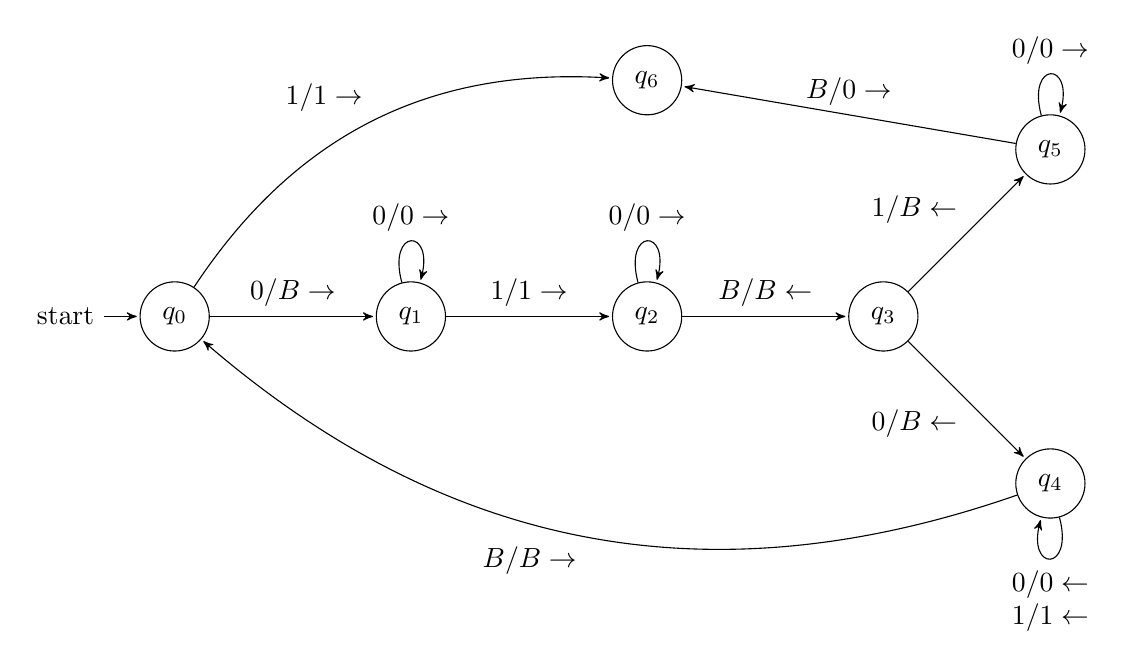
\begin{tikzpicture}[>=stealth',shorten >=1pt,auto,node distance=3cm]
 \node[initial,state] (q0) {$q_0$};
 \node[state,right of=q0] (q1) {$q_1$};
 \node[state,right of=q1] (q2) {$q_2$};
 \node[state,right of=q2] (q3) {$q_3$};
 \node[state,below right of=q3] (q4) {$q_4$};
 \node[state,above right of=q3] (q5) {$q_5$};
 \node[state,above of=q2] (q6) {$q_6$};

 \draw [->]
 (q0)
 edge node {$0 / B \rightarrow$} (q1)
 edge [bend left] node {$1 / 1 \rightarrow$} (q6)
 (q1)
 edge node {$1 / 1 \rightarrow$} (q2)
 edge [loop above] node {$0 / 0 \rightarrow$} (q1)
 (q2)
 edge node {$B / B \leftarrow$} (q3)
 edge [loop above] node {$0 / 0 \rightarrow$} (q2)
 (q3)
 edge node [below left] {$0 / B \leftarrow$} (q4)
 edge node {$1 / B \leftarrow$} (q5)
 (q4)
 edge [bend left] node {$B / B \rightarrow$} (q0)
 edge [loop below] node {$
 \begin{array}{c}
 0 / 0 \leftarrow \\
 1 / 1 \leftarrow
 \end{array}$} (q4)
 (q5)
 edge node [above] {$B / 0 \rightarrow$} (q6)
 edge [loop above] node {$0 / 0 \rightarrow$} (q5);
 \end{tikzpicture}
 \caption{第一题}
 \end{figure}
\end{solution}

\section{第二题}
Let x and y are positive numbers.
Please design a Turing Machine (diagram) to compute $x \div y$ (x divisible by y).
You should explain the notation of x and y.
Hint: you may get the notation as simple as you can.

\begin{solution}
 我们使用字符$0$来表示$x$和$y$,
 利用$0^n$来表示数$n$,用$B$来间隔。
 具体的说,
 纸带上开始是$\cdots 0^x B 0^y \cdots$。
 最终纸带上的字符是$\cdots 0^{x \div y} \cdots$,
 由于图太大,此处给处转移表,其中$q_{40}$为接收状态。
 \begin{table}[H]
 \vspace{0.5em}\centering\wuhao{}
 \begin{tabular}{l|cc}
 \multirow{2}{*}{状态}
 & \multicolumn{2}{c}{符号}                    \\
 ~        & B                        & 0                \\
 \toprule                                               \\
 $q_{0}$  & ($q_{0}$, B, R)          & ($q_{1}$, 0, L)  \\
 $q_{1}$  & ($q_{2}$, B, L)          & ($q_{2}$, B, L)  \\
 $q_{2}$  & ($q_{3}$, 0, L)          & ($q_{3}$, 0, L)  \\
 $q_{3}$  & ($q_{4}$, B, R)          & ($q_{4}$, B, R)  \\
 $q_{4}$  & ($q_{5}$, 0, R)          & ($q_{5}$, 0, R)  \\
 $q_{5}$  & ($q_{6}$, B, R)          & ($q_{40}$, 0, L) \\
 $q_{6}$  & ($q_{7}$, B, R)          & ($q_{6}$, 0, R)  \\
 $q_{7}$  & ($q_{7}$, B, R)          & ($q_{8}$, B, R)  \\
 $q_{8}$  & ($q_{23}$, B, L)         & ($q_{9}$, 0, L)  \\
 $q_{9}$  & ($q_{9}$, B, L)          & ($q_{10}$, 0, L) \\
 $q_{10}$ & ($q_{11}$, B, R)         & ($q_{37}$, 0, L) \\
 $q_{11}$ & ($q_{40}$, B, L)         & ($q_{12}$, 0, R) \\
 $q_{12}$ & ($q_{12}$, B, R)         & ($q_{13}$, 0, L) \\
 $q_{13}$ & ($q_{14}$, 0, L)         & ($q_{40}$, 0, L) \\
 $q_{14}$ & ($q_{15}$, B, L)         & ($q_{40}$, 0, L) \\
 $q_{15}$ & ($q_{16}$, B, L)         & ($q_{19}$, 0, L) \\
 $q_{16}$ & ($q_{16}$, B, L)         & ($q_{17}$, 0, L) \\
 $q_{17}$ & ($q_{18}$, 0, R)         & ($q_{17}$, 0, L) \\
 $q_{18}$ & ($q_{12}$, B, R)         & ($q_{18}$, 0, R) \\
 $q_{19}$ & ($q_{20}$, B, L)         & ($q_{19}$, 0, L) \\
 $q_{20}$ & ($q_{20}$, B, L)         & ($q_{21}$, 0, L) \\
 $q_{21}$ & ($q_{22}$, B, R)         & ($q_{21}$, 0, L) \\
 $q_{22}$ & ($q_{40}$, B, L)         & ($q_{40}$, B, L) \\
 $q_{23}$ & ($q_{23}$, 0, L)         & ($q_{24}$, 0, R) \\
 $q_{24}$ & ($q_{40}$, B, L)         & ($q_{25}$, B, L) \\
 $q_{25}$ & ($q_{40}$, B, L)         & ($q_{26}$, 0, L) \\
 $q_{26}$ & ($q_{32}$, B, R)         & ($q_{27}$, 0, L) \\
 $q_{27}$ & ($q_{39}$, B, L)         & ($q_{27}$, 0, L) \\
 $q_{28}$ & ($q_{29}$, 0, L)         & ($q_{28}$, 0, L) \\
 $q_{29}$ & ($q_{30}$, B, R)         & ($q_{30}$, B, R) \\
 $q_{30}$ & ($q_{31}$, B, R)         & ($q_{30}$, 0, R) \\
 $q_{31}$ & ($q_{31}$, B, R)         & ($q_{6}$, B, R)  \\
 $q_{32}$ & ($q_{40}$, B, L)         & ($q_{33}$, B, R) \\
 $q_{33}$ & ($q_{34}$, B, R)         & ($q_{40}$, 0, L) \\
 $q_{34}$ & ($q_{35}$, B, L)         & ($q_{34}$, B, R) \\
 $q_{35}$ & ($q_{35}$, B, L)         & ($q_{36}$, 0, L) \\
 $q_{36}$ & ($q_{40}$, B, L)         & ($q_{36}$, 0, L) \\
 $q_{37}$ & ($q_{38}$, B, R)         & ($q_{37}$, 0, L) \\
 $q_{38}$ & ($q_{40}$, B, L)         & ($q_{6}$, B, R)  \\
 $q_{39}$ & ($q_{39}$, B, L)         & ($q_{28}$, 0, L) \\
 $q_{40}$ & ---                      & ---
 \end{tabular}
 \end{table}

\end{solution}

\section{第三题}
Show that the regular languages are closed under the following operations:
\[
 \min(L) = \{ w | w \text{ is in $L$, but no proper prefix of $w$ is in } L \}
\]

\begin{proof}
 所有不合法的语言为$L\Sigma^+$,
 所以$\min(L) = L - L\Sigma^+$。
 由于正则语言对于连接和差运算满足封闭性,
 所以$L\Sigma^+$是正则语言,
 $\min(L) = L - L\Sigma^+$是正则语言。
\end{proof}

\section{第四题}
Use the CFL pumping lemma to show that the following language is not context free:
\[
 \{ a^i b^j c^k | i < j < k \}
\]

\begin{proof}
 假设$L$是一个 CFL,
 根据泵引理,存在一个对应的常正整数$n$。

 考虑字符串$s = a^{n}b^{n + 1}c^{n + 2}$。
 根据泵引理,我们将$s$分割为$s = uvwxy$,
 其中$|vwx| \le n, vx \neq \varepsilon$。
 考虑下面两种情况
 \begin{enumerate}[fullwidth,itemindent=\parindent,label=(\arabic*)]
 \item
 $vwx$ 不包含字符$a$,
 那么$uv^0wx^0y$中的长度$ \le 2n + 3$,
 又由于$n \ge 1$,
 所以不可能存在$j, k$,满足
 $n < j < k, j + k \le 2n + 3$。
 \item
 $vwx$包含字符$a$,
 那么$uv^9wx^9y$中$a$或$b$的个数必定大于$c$的,
 所以$uv^9wx^9y \notin L$。
 \end{enumerate}

 综上所述,$L$不是一个 CFL。
\end{proof}

\section{第五题}
Give a context-free grammar for the following language over
the alphabet $ \Sigma = \{a, b\}$:
\[
 L = \{a^i b^j | i \neq j~and~i \neq 2j \}
\]

\begin{solution}
 我们定义一个 CFG $G = (\{S, A, B, C, X, Y, Z\}, \{a, b\}, P, S)$,其中$P$为
 \begin{align*}
 S & \to A | B | C               \\
 A & \to Xb                      \\
 X & \to Xb | aXb | \varepsilon  \\
 B & \to aaYbbb                  \\
 Y & \to aYb | aaYb              \\
 C & \to aZ                      \\
 Z & \to aZ | aaZb | \varepsilon
 \end{align*}
\end{solution}

\end{document}
